\lecture{Detecção probabilística}{lec_eqz}

\begin{frame}
	\begin{block}{\centering\large\bfseries Parte 5}
		\centering\large\insertpart
	\end{block}
\end{frame}

\section{Detecção probabilística}

\begin{frame}
	\frametitle{Detecção probabilística}

	\begin{itemize}
	    \item Projeto do receptor baseado em distância mínima:
	    \begin{itemize}
	      \item Robusto na presença de ruído.
	      \item Questões: quando o receptor é ótimo? o que fazer quando não é ótimo?
	    \end{itemize}
	    \item Teoria da detecção ótima:
	    \begin{itemize}
	      \item Identificação das circunstâncias nas quais o receptor de distância mínima é ótimo.
	      \item Aplicação para canais discretos e contínuos no tempo.
	      \item Caracterização probabilística.
	    \end{itemize}
	    \item Notação: variáveis aleatórias com letras maiúsculas (como $X$) e valores determinísticos com letras minúsculas (como $x$).
	    \item Processamento determinístico (geração de sinal) e processamento estatístico (geração de ruído).
	    \begin{figure}[t]	
	      \begin{center}
		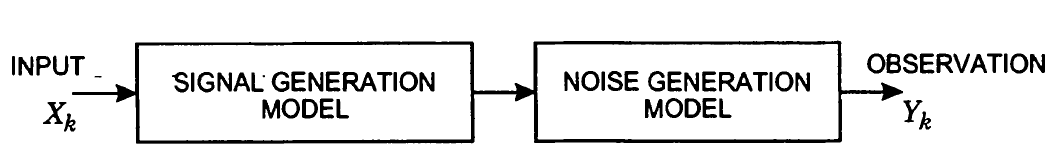
\includegraphics[width=0.65\columnwidth]{figs/detec_01}
	      \end{center}
	    \end{figure}
	\end{itemize}			
\end{frame}


\section{Detecção de um sinal real}

\begin{frame}
	\frametitle{Detecção de um sinal real}

	\begin{itemize}
	    \item Caso simplificado:
	    \begin{itemize}
	      \item A entrada é uma variável aleatória $X \in \mathcal{A}$.
	      \item O gerador de sinal repassa esse símbolo diretamente para o gerador de ruído.
	      \item A saída pode ser uma observação com valores $Y$ discretos ou contínuos.
	    \end{itemize}
	    \item Observação de valores discretos:
	    \begin{itemize}
	      \item Para projetar o detector, devemos conhecer a distribuição $p_{Y|A}(y|\hat{a})$.
	      \item \textbf{Detector de Máxima Verossimilhança} (ML - \textit{Maximum Likelihood}).
	      \item Detector ML escolhe o $\hat{a}\in \mathcal{A}$ que maximiza $p_{Y|A}(y|\hat{a})$.
	      \item Vantagem da detecção ML: a verossimilhança pode ser calculada facilmente para cada $\hat{a}$, conhecendo apenas as estatísticas do gerador de ruído.
	    \end{itemize}
	\end{itemize}			
\end{frame}

\begin{frame}
	\frametitle{Observações discretas}

	\begin{itemize}
	    \item Exemplo de detector ML:
	    \begin{itemize}
	      \item Considere $Y= A + N$, onde $A$ e $N$ são independentes e assumem valores 0 ou 1 (lançamento de moeda não-viciada).
	      \item Possíveis observações: $y=$ 0, 1 ou 2.
	      \item Cálculo da verossimilhança:
	    \end{itemize}
	    \begin{align*}
		p_{Y|A}(0|\hat{a}) &= \begin{cases}
					0,5  \quad &\text{para } \hat{a}=0 \\
					0 \quad &\text{para } \hat{a}=1
		                      \end{cases} \\
		p_{Y|A}(1|\hat{a}) &= \begin{cases}
					0,5  \quad &\text{para } \hat{a}=0 \\
					0,5 \quad &\text{para } \hat{a}=1
		                      \end{cases} \\
		p_{Y|A}(2|\hat{a}) &= \begin{cases}
					0  \quad &\text{para } \hat{a}=0 \\
					0,5 \quad &\text{para } \hat{a}=1
		                      \end{cases}
	    \end{align*}


	\end{itemize}			
\end{frame}

\begin{frame}
	\frametitle{Observações discretas}

	\begin{itemize}
	    \item Detector de máxima probabilidade a posteriori (MAP):
	    \begin{itemize}
	      \item Maximiza a probabilidade posterior $p_{A|Y}(\hat{a}|y)$.
	      \item O receptor MAP minimiza a probabilidade de erro.
	      \item Também chamada de detecção Bayesiana.
	      \item Regra de Bayes:
	      \begin{equation*}
		  p_{A|Y}(\hat{a}|y) = \frac{p_{Y|A}(y|\hat{a}) p_A(\hat{a})}{p_Y(y)}
	      \end{equation*}
	      \item É necessário o conhecimento das probabilidades a priori $p_A(\hat{a})$.
	      \item Para o caso em que as probabilidades a priori assumem o mesmo valor, o critério MAP recai no critério ML.
	    \end{itemize}
	    \item Canal binário simétrico (BSC):
	    \begin{figure}[t]	
	      \begin{center}
		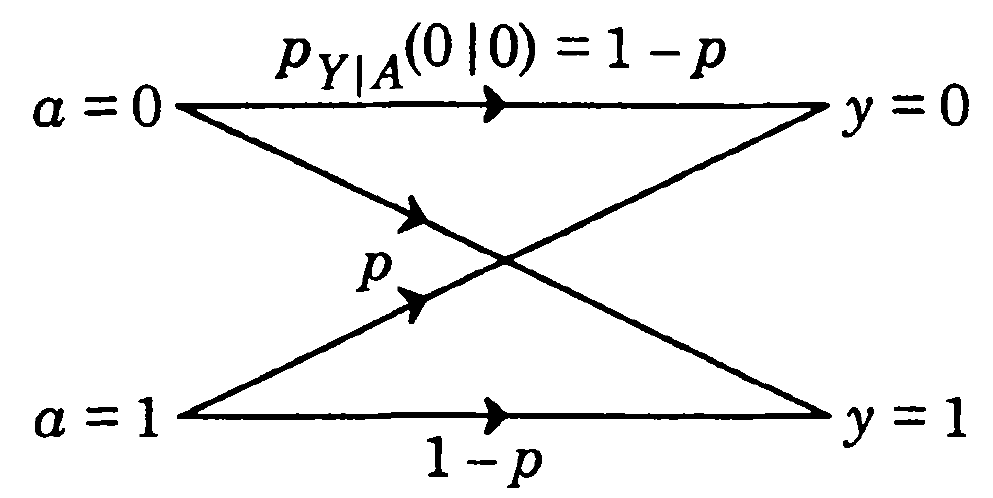
\includegraphics[width=0.35\columnwidth]{figs/detec_02}
	      \end{center}
	    \end{figure}
	\end{itemize}			
\end{frame}

\begin{frame}
	\frametitle{Observações contínuas}

	\begin{itemize}
	    \item O modelo mais comum de ruído $N$ corrompe os símbolos de entrada com valores contínuos.
	    \item A observação $Y=A+N$ é portanto uma variável aleatória contínua.
	    \item Critério MAP utilizando a forma mista de Bayes:
	    \begin{equation*}
		  p_{A|Y}(\hat{a}|y) = \frac{f_{Y|A}(y|\hat{a}) p_A(\hat{a})}{f_Y(y)}
	      \end{equation*}
	      \item Exemplos:
	    \begin{figure}[t]	
	      \begin{center}
		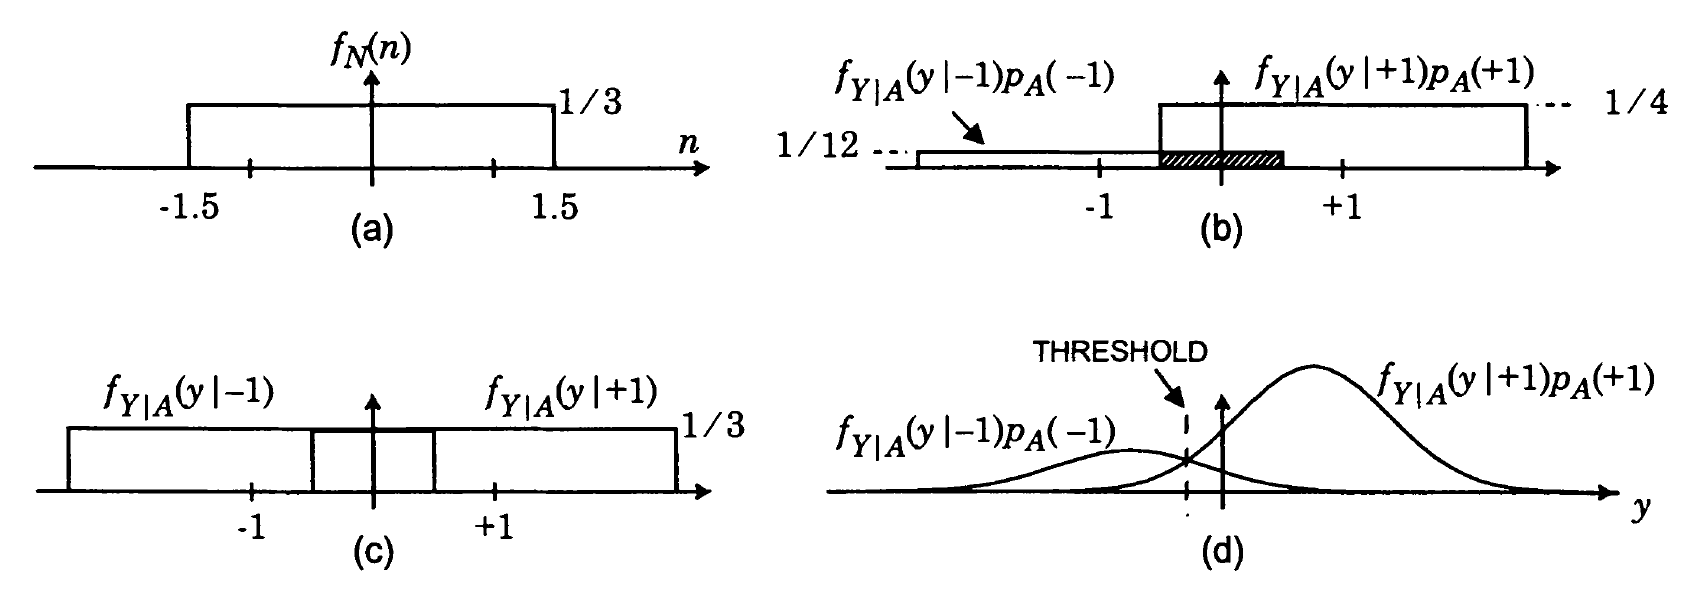
\includegraphics[width=0.8\columnwidth]{figs/detec_03}
	      \end{center}
	    \end{figure}
	\end{itemize}			
\end{frame}

\section{Detecção de um vetor de sinal}

\begin{frame}
	\frametitle{Detecção de um vetor de sinal}

	\begin{itemize}
	    \item Modelo de comunicação vetorial:
	    \begin{figure}[t]	
	      \begin{center}
		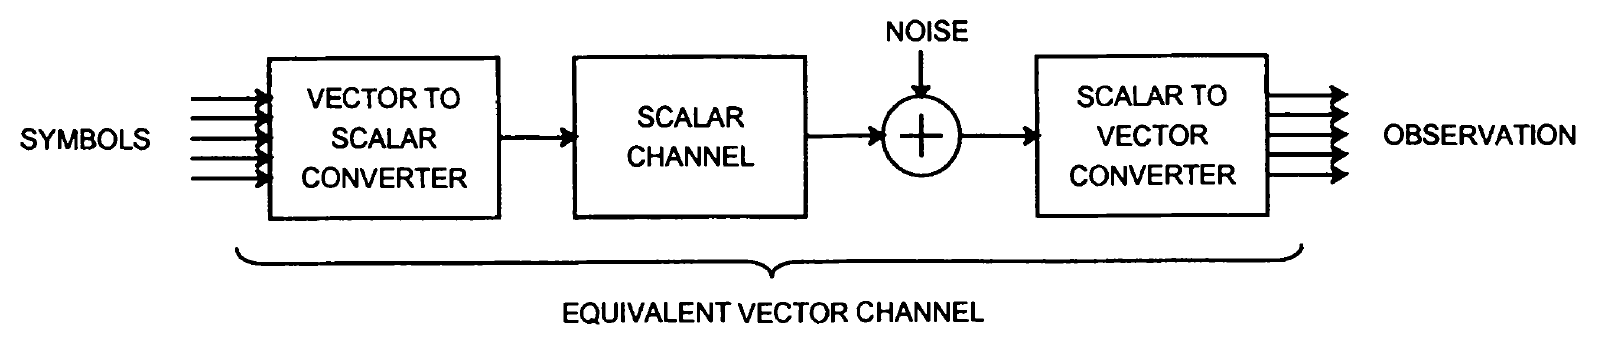
\includegraphics[width=0.8\columnwidth]{figs/detec_04}
	      \end{center}
	    \end{figure}
	    \item O gerador de sinal aceita uma entrada $X$, a qual é mapeada em um vetor de sinal $\mathbf{S}$ com dimensão $N$.
	    \item A observação é um vetor $\mathbf{Y}$ com mesma dimensão do sinal.
	    \item Distribuição condicional da observação: $f_{\mathbf{Y}|\mathbf{S}}(\mathbf{y}|\mathbf{s})$.
	    \item O detector decide qual o vetor $\hat{\mathbf{s}}$ que foi de fato transmitido.
	    \item Caso em que as componentes do ruído são independentes:
	    \begin{equation*}
		f_{\mathbf{Y}|\mathbf{S}}(\mathbf{y}|\mathbf{s}) = \prod_{k=1}^N f_{Y_k|S_k}(y_k|s_k)
	    \end{equation*}

	\end{itemize}			
\end{frame}

\begin{frame}
	\frametitle{Detecção ML vetorial}

	\begin{itemize}
	    \item Considere o canal AWGN: $\mathbf{Y} = \mathbf{S} + \mathbf{N}$.
	    \item Os elementos de $\mathbf{S}$ são escolhidos dentre $M$ possibilidades.
	    \item E $\mathbf{N}$ é um vetor de ruído complexo Gaussiano circularmente simétrico, com componentes independentes e de variância $2\sigma^2$.
	    \item Expressão para a função densidade de probabilidade:
	    \begin{equation*}
		f_{\mathbf{Y}|\mathbf{S}}(\mathbf{y}|\mathbf{s}) = f_{\mathbf{N}}(\mathbf{y}-\mathbf{s})
	    \end{equation*}
	    \item Componentes do ruído:
	    \begin{equation*}
		f_{\mathbf{N}}(\mathbf{n}) = \prod_{k=1}^N f_{N_k}(n_k) = \prod_{k=1}^N \frac{1}{2\pi \sigma^2} e^{-|n|^2/2\sigma^2} = \frac{1}{(2\pi \sigma^2)^N} e^{-||\mathbf{n}||^2/2\sigma^2}
	    \end{equation*}
	    \item Maximizar $f_{\mathbf{N}}(\mathbf{y}-\hat{\mathbf{s}})$ é equivalente a minimizar $||\mathbf{y} - \hat{\mathbf{s}} ||^2$.
	\end{itemize}			
\end{frame}

\begin{frame}
	\frametitle{Detecção ML vetorial}

	\begin{itemize}
	    \item Para o canal binário simétrico (BSC) temos que:
	    \begin{equation*}
		P_{Y_k | S_k} (y|\hat{s}) = \begin{cases}
						p &\quad y \neq \hat{s} \\
						1-p &\quad y = \hat{s}
		                            \end{cases}
	    \end{equation*}
	    \item Definição da distância de Hamming $d_H(\hat{\mathbf{s}}, \mathbf{y})$: número de componentes distintas entre os vetores binários.
	    \item Distribuição condicional conjunta:
	    \begin{equation*}
		P_{\mathbf{Y} | \mathbf{S}} (\mathbf{y}|\hat{\mathbf{s}}) = p^{d_H(\hat{\mathbf{s}}, \mathbf{y})}(1-p)^{N - d_H(\hat{\mathbf{s}}, \mathbf{y})} = (1-p)^N \left(\frac{p}{1-p} \right)^{d_H(\hat{\mathbf{s}}, \mathbf{y})}
	    \end{equation*}
	    \item Para $p < 1/2$, o detector ML escolhe o $\hat{\mathbf{s}}$ que minimiza a distância de Hamming.
	\end{itemize}			
\end{frame}

\begin{frame}
	\frametitle{Detecção MAP vetorial}

	\begin{itemize}
	    \item O detector MAP é mais complicado e requer conhecimento extra sobre a estatística do ruído.
	    \item Assumindo que as probabilidades a priori $p_{\mathbf{S}}(\hat{\mathbf{s}})$ são conhecidas, temos o critério MAP vetorial:
	    \begin{equation*}
		p_{\mathbf{S}|\mathbf{Y}}(\hat{\mathbf{s}}|\mathbf{y}) = \frac{f_{\mathbf{Y}|\mathbf{S}}(\mathbf{y}|\hat{\mathbf{s}}) p_{\mathbf{S}}(\hat{\mathbf{s}})}{f_{\mathbf{Y}}(\mathbf{y})}
	    \end{equation*}
	    \item Como o denominador é independente de $\hat{\mathbf{s}}$, o critério MAP equivale a maximizar o numerador.
	    \item Recai no ML para o caso em que as probabilidades a priori são iguais.
	\end{itemize}			
\end{frame}

\section{Sinais conhecidos em ruído Gaussiano}

\begin{frame}
	\frametitle{Sinal recebido discreto no tempo}

	\begin{itemize}
	    \item Modelo do sinal recebido:
	    \begin{equation*}
		Y_k = s_k^{(m)} + N_k \, , \qquad 0 \leq k \leq \infty
	    \end{equation*}
	    \item Função custo otimizada pelo detector ML:
	    \begin{equation*}
		J_m = \sum_{k=0}^{\infty} \left|Y_k - s_k^{(m)} \right|^2 = \sum_{k=0}^{\infty} \left|Y_k \right|^2 + \sum_{k=0}^{\infty} \left| s_k^{(m)} \right|^2 - 2 \mathrm{Re} \left\{\sum_{k=0}^{\infty} Y_k s_k^{(m)*} \right\}
	    \end{equation*}
	    \item Escolha do $m$ que minimiza a expressão. O critério ML é equivalente a maximizar:
	    \begin{equation*}
		R_m = \mathrm{Re}\left\{\sum_{k=0}^{\infty} Y_k s_k^{(m)*} \right\} - \frac{1}{2}\mathcal{E}_m
	    \end{equation*}

	\end{itemize}			
\end{frame}

\begin{frame}
	\frametitle{Recepção contínua no tempo}

	\begin{itemize}
	    \item Modelo do sinal recebido:
	    \begin{small}
	    \begin{equation*}
		Y(t) = s_m(t) + N(t) \, , \qquad 0 \leq t < T
	    \end{equation*}
	    \end{small}
	    \item $N(t)$ é um processo Gaussiano estacionário circularmente simétrico, de média zero, com DEP $S_N(f)$ e autocorrelação $R_N(\tau)$.
	    \item Para realizar a detecção, o problema tem que ser tornado equivalente ao caso discreto. Abordagem de expansão do espaço de sinais em termos de funções ortonormais:
	    \begin{small}
	    \begin{align*}
		N(t) &= \sum_{i=1}^{\infty} N_i \phi_i(t) \, , \qquad \text{para } \int_0^T \phi_i(t)\phi_j^*(t)dt = \delta_{i-j} \\
		Y(t) &= \sum_{i=1}^{\infty} Y_i \phi_i(t)
	    \end{align*}
	    \end{small}
	    \item Assumindo que os coeficientes são descorrelacionados: $\mathrm{E}[N_iN_j^*] = \sigma_i^2 \delta_{i-j}$, é possível encontrar um conjunto de funções ortonormais que satisfazem essa condição.
	\end{itemize}			
\end{frame}

\begin{frame}
	\frametitle{Recepção contínua no tempo}

	\begin{itemize}
	    \item Expansão de Karhunen-Loeve:
	    \begin{equation*}
		N_j = \int_0^T N(t) \phi_j^*(t) dt  \, , \qquad s_i^{(m)} = \int_0^T s_m(t) \phi_i^*(t) dt
	    \end{equation*}
	    \item O sinal contínuo pode ser expresso em uma forma equivalente discreta:
	    \begin{equation*}
		\frac{Y_i}{\sigma_i} = \frac{s_i^{(m)}}{\sigma_i} + \frac{N_i}{\sigma_i} \, , \qquad 1 \leq i < \infty
	    \end{equation*}
	    \item A normalização é necessária, pois as componentes de ruído não possuem necessariamente a mesma variância $\mathrm{E}[|N_i|^2] = \sigma_i^2$.
	\end{itemize}			
\end{frame}

\begin{frame}
	\frametitle{Recepção contínua no tempo}

	\begin{itemize}
	    \item O detector ML para essa representação equivalente minimiza:
	    \begin{equation*}
		J_m = \sum_{i=1}^{\infty} \left|\frac{Y_i}{\sigma_i} - \frac{s_i^{(m)}}{\sigma_i}  \right|^2 = \sum_{i=1}^{\infty} \frac{\left|Y_i - s_i^{(m)}\right|^2}{\sigma_i^2}
	    \end{equation*}
	    \item De forma análoga, o detector ML maximiza a correlação:
	    \begin{equation*}
		R_m = \mathrm{Re}\left\{\sum_{i=1}^{\infty} \frac{Y_is_i^{(m)*}}{\sigma_i^2} \right\} - \frac{1}{2}\mathcal{E}_m
	    \end{equation*}
	    \item Foi demonstrado que o sinal recebido contínuo de infinitas dimensões pode ser reduzido a um conjunto de $M$ variáveis de decisão $R_m$.
	\end{itemize}			
\end{frame}

\section{Detecção de máxima verossimilhança}

\begin{frame}
	\frametitle{Detecção de máxima verossimilhança com algoritmo de Viterbi}

	\begin{itemize}
	    \item Demonstramos anteriormente que o algoritmo de Viterbi pode resolver o problema de detecção em sequência de mínima distância.
	    \item Ele também pode ser generalizado para a detecção em sequência de máximo verossimilhança (ML), para qualquer gerador de sinal de Markov e qualquer gerador de ruído com componentes independentes.
	    \item Definições:\vspace{-0.2cm}
	    \begin{align*}
		    Q &\text{ estados, } \{0,\ldots,Q-1 \} \\
		    L &\text { símbolos de entrada, } \{a_0,\ldots, a_{L-1} \} \text{, com } a\in \mathcal{A} \\
		    \mu &\text{ símbolos inativos} \\
		    \Psi &= [ \Psi_0, \ldots, \Psi_{L+\mu} ] \in \{0,\ldots,Q-1 \}^{L+\mu+1} \, : \text{ sequência de estados} \\
		    \mathbf{Y} &= [Y_0, \ldots, Y_{L+\mu-1}] \, : \text{ vetor de observações ruidosas}
	    \end{align*}
	    \item O número de observações é menor que o tamanho da sequência de estados, pois corresponde às \textit{transições} entre estados.
	\end{itemize}			
\end{frame}

\begin{frame}
	\frametitle{Detecção de máxima verossimilhança com algoritmo de Viterbi}

	\begin{itemize}
	    \item Dada uma observação $\mathbf{y}$, o detector em sequência MAP seleciona o vetor $\boldsymbol{\psi}$ que maximiza $p_{\Psi | \mathbf{Y}}(\boldsymbol{\psi}|\mathbf{y}) = p(\boldsymbol{\psi}|\mathbf{y})$.
	    \item O critério MAP pode de forma equivalente maximizar o produto $p(\boldsymbol{\psi}|\mathbf{y})f(y)$ ou $f(\mathbf{y}|\boldsymbol{\psi})p(\boldsymbol{\psi})$.
	    \item Podemos demonstrar que:
	    \begin{equation*}
		f(\mathbf{y}|\boldsymbol{\psi})p(\boldsymbol{\psi}) = \prod_{k=0}^{L+\mu-1} \left[ f(y_k|\psi_k , \psi_{k+1})p(\psi_{k+1}|\psi_k) \right]
	    \end{equation*}
	    \item Essa é uma \textit{métrica de caminho}, igual ao produto das \textit{métricas de ramo}, relativas à transição de $\psi_k$ para $\psi_{k+1}$.
	    \item Semelhante ao algoritmo visto anteriormente, com uma ligeira diferença para tratar uma métrica de ramo multiplicativa.
	\end{itemize}			
\end{frame}


